\documentclass[12pt,reqno]{amsart}
\usepackage{fullpage}
\usepackage{amsfonts}
\usepackage{amssymb}
\usepackage{times}
\usepackage{graphicx}
\usepackage{mathtools}
\usepackage{breakurl}
\usepackage{bm}
\usepackage{url}
\usepackage[all]{xy}
\usepackage[margin=0.8in,footskip=0.25in]{geometry}
\usepackage[all]{xy}
\usepackage{tikz}

\usepackage[colorlinks=true,
            linkcolor=red,
            urlcolor=blue,
            citecolor=gray]{hyperref}
\vfuzz=2pt


\DeclarePairedDelimiter\ceil{\lceil}{\rceil}
\DeclarePairedDelimiter\floor{\lfloor}{\rfloor}

\DeclareMathOperator{\cok}{coker}
\DeclareMathOperator{\im}{im}
\DeclareMathOperator{\ann}{Ann}
\DeclareMathOperator{\Hom}{Hom}


% some "funny lines" referred to later:
\newtheorem{theorem}{Theorem}[section]
\newtheorem{corollary}[theorem]{Corollary}
\newtheorem{lemma}[theorem]{Lemma}
\newtheorem{proposition}[theorem]{Proposition}
{\theoremstyle{remark}\newtheorem*{remark}{Remark}}
\theoremstyle{definition}
\newtheorem{definition}[theorem]{Definition}
\newtheorem{example}[theorem]{Example}


\newcommand{\lex}{\mbox{lexdeg}}
\newcommand{\mymod}[3]{#1 \equiv #2 \Mod{#3}}
\newcommand{\ccc}{\mathcal{C}}
\newcommand{\nmm}[2]{\text{N}_{#1}(#2)}
\newcommand{\Mod}[1]{\ (\mathrm{mod}\ #1)}
\newcommand{\gal}{\text{Gal}}
\newcommand{\cc}{\mathbb{C}}
\newcommand{\zz}{\mathbb{Z}}
\newcommand{\ta}[1]{\langle #1 \rangle}
\newcommand{\ff}{\mathbb{F}}
\newcommand{\qq}{\mathbb{Q}}
\newcommand{\Tor}[2]{\mathbf{Tor}_{#1}(#2)}
\newcommand{\sqrtn}[1]{\sqrt[n]{#1}}
\newcommand{\charr}{\text{char}}
\newcommand{\disc}[1]{\mbox{disc}(#1)}
\newcommand{\Aut}{\text{Aut}}
\newcommand{\Inn}{\text{Inn}}
\newcommand{\Gal}{\text{Gal}}
\newcommand{\sgn}{\text{sgn}}
\newcommand{\irr}{\text{irr}}
\newcommand{\of}{\overline{F}}
\newcommand{\ok}{\overline{K}}
\newcommand{\ZZ}{\mathbb{Z}}
\newcommand{\NN}{\mathbb{N}}
\newcommand{\CC}{\mathbb{C}}
\newcommand{\QQ}{\mathbb{Q}}
\newcommand{\RR}{\mathbb{R}}
\newcommand{\FF}{\mathbb{F}}
\newcommand{\Tr}{\text{Tr}}
\newcommand{\nm}{\text{N}}
\newcommand{\tk}{\theta_K}
\newcommand{\mm}{\mathfrak{m}}
\newcommand{\tor}{\mathbf{Tor}}
\newcommand{\conv}[1]{\mathrm{conv}(#1)}
\newcommand{\diam}[1]{\mathrm{diam}(#1)}
\newcommand{\vol}[1]{\mathrm{vol}(#1)}
\newcommand{\la}{\langle}
\newcommand{\ra}{\rangle}

\begin{document}

\title{HW3}

\noindent \textbf{Q1:} (a): Set   $$X=\{(0,0),(1,2),(2,1),(3,22),(4,20),(5,21)\}$$ as drawn in the picture.

\begin{center}
  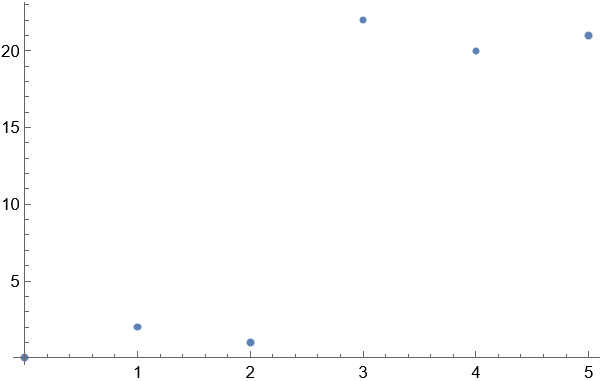
\includegraphics[scale=0.4]{pentagon.png}
\end{center} And we can use brute force to check there is no 4-cup and no 4-cap. Or we can see this from the proof in part (b).\\


(b): For simplicity, we set $f(k,l)=\binom{k+l-4}{k-2}$. If either $k$ or $l$ is 2, then $f(k,l)=1$. It is clear that we cannot get a 2-cup or a 2-cap out of only 1 point. $f(3,3)=2$ and it is also clear that we cannot get a 3-cup or 3-cap out of 2 points. Assume $k,l\geq 3$. Now to get a configuration of $f(k,l)$ points with no $k$-cup and no $l$-cup, we construct by double induction.


The base case is $f(4,3)=f(3,4)=3$. It is clear that 3 points forming a 3-cup serve as a configuration of 3 points points with no 4-cup and no 3-cap, and 3 points forming a 3-cap serve as a configuration of 3 points points with no 3-cup and no 4-cap.

The double inductive construction goes as follows. Let $X$ be a configuration of $f(k-1,l)$ points with no $(k-1)$-cup and no $l$-cap, and $Y$ be a configuration of $f(k,l-1)$ points with no $k$-cup and no $(l-1)$-cap. Then they are only finitely many slopes we can get from joining points in $X$ to points in $X$ and points in $Y$ to points in $Y$.
\begin{center}
  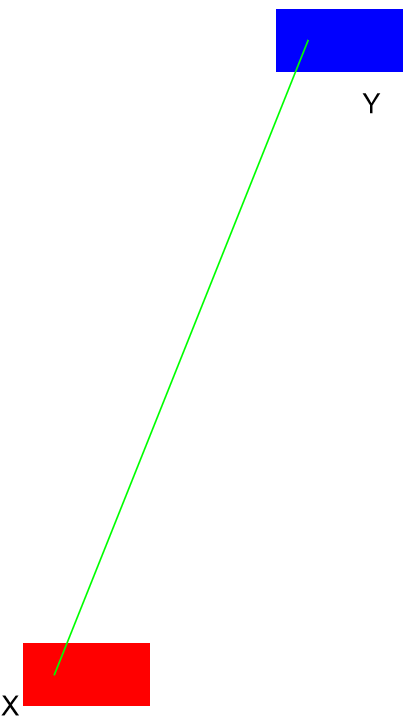
\includegraphics[scale=0.4]{no_cup_cap.png}
\end{center}
Now we put $Y$ (actually, a translated copy of $Y$) far above $X$ to its right as shown in the picture in such a way that the slope of any line connecting a point in $X$ with a point in $Y$ is greater than the slopes we can get from joining points in $X$ to points in $X$ and points in $Y$ to points in $Y$. We claim this new configuration $Z=X\cup Y$, which consists of $f(k-1,l)+f(k,l-1)=f(k,l)$ points, has no $k$-cup and no $l$-cap. We argue that there is no $k$-cup and the non-existence of $l$-cap is similar.

If there exists a $k$-cup $C$, then $C$ must consist of points both from $X$ and $Y$ by the assumptions on $X$ and $Y$. However, if $C$ contains more than two points from $Y$, then the slope of the line joining these two points in $Y$ is less than the slope of the line joining the right most point of $C\cap X$ to the left most point of $C\cap Y$, which cannot happen in a $k$-cup. Hence we have $|C\cap X|=k-1$ and $|C\cap Y|=1$. But this implies $C\cap X$ is a $(k-1)$-cap and contradicts to the assumptions on $X$.


\newpage

\noindent \textbf{Q2:} For $n \geq 3$, let $f(n)$ be the minimum number so that if $f(n)$ points are in the plane in general position, then there exist $n$ of these point forming a convex $n$-gon. By the Erd\H{o}s-Szekeres theorem, $f(n)$ exits.


We claim $n(k)=R_3(k,f(k))$, where the symbol $R_r(k,l)$ is the Ramsey number for $r$-sets (as in lecture slides), serves the purpose in this problem. For any $N\geq R_3(k,f(k))$ points on the plane, we colour the 3-sets of $N$ as follows: a 3-set is coloured to be red if these 3 points are collinear and coloured blue if they are not collinear, i.e., in general position. Then by the Ramsey's theorem for $r$-sets, there exists either a set of $k$ points with all 3-sets red or a set of $f(k)$ points with all 3-sets blue. If it is the former, there these $k$ points are collinear since every 3 of them are collinear (as all its 3-sets are red). If it is the latter, then these $f(k)$ points are in general position since no 3 of them are collinear; but then by the Erd\H{o}s-Szekeres theorem, there is a $k$-gon whose vertices are in the point set. Both the cases, we are done.

% We claim $n(k)=kf(k)$ serves the purpose in this problem --- actually, this is an overkill. Let $X$ be an arbitrary configuration of $kf(k)$ points in the plane. If there are $k$ points from $X$ lying on a common line, we are done. Now assume there are at most $k-1$ points on any line on the plane. Note $|X|=kf(k)\geq  k^2$. Consider the collection of subsets of $X$ which consists of more than two elements lying on the same line, namely,
% $$P_0=\{A\subset X: |A|\geq 2 \mbox{ and all points of }A\mbox{ lie on the same line}\}.$$
% Then $P_0$ is finite and nonempty since any two points determines a line. Take $X_1$ from $P_0$ of the maximum cardinality --- there might be many choices, but just pick any one. By assumption, $|S_1|<k$.

% Set $X_1=X-S_0$ and so $|X_1| = |X|-|S_0| > kf(k)-k =k(f(k)-1) > k(k-1)$. Repeat the construction to get $S_2$. That is, we consider
% $$P_1=\{A\subset X_1: |A|\geq 2 \mbox{ and all points of }A\mbox{ lie on the same line}\}$$ and take $S_2$ from $P_1$ of the maximum cardinality. Then we also have $|S_1|<k$.

% Keep repeating the procedure until we have $f(k)$ of $S_i$'s, that is, we construct $S_1, S_2,\dots, S_{f(k)}$. This is doable because each $|S_i|<k$ and $|X_i|>k(f(k)-i))$. Now take 2 points $x_i, y_i$ from each $S_i$. We claim $x_1,y_1,x_2,y_2,\dots,x_{f(k)},y_{f(k)}$ are in general position. If not


\newpage

\noindent \textbf{Q3:} Colour the origin 0 to be red. The plane is the union of all the straight lines that pass through 0. For any line passing through the origin, choose either green or blue. Colour the whole of the lines, except the origin 0, with the selected colour. Indeed, we colour those of rational slope with green and those of irrational slope with blue.

An arbitrary line in the plane, if it passes through the origin, is coloured with either red/green or red/blue. If a line does not pass through the origin, it contains only green and blue points. And it must contain both green and blue points since the slopes of the line segments connecting a point on the line to the origin can be achieved to be irrational and/or rational.


\newpage

\noindent \textbf{Q4:} Say the colours we use are red and blue. Since for any positive distance $d$, we know from lecture that a pair of monochromatic points of distance $d$ can be achieved. (Namely, consider an equilateral triangle of edge length $d$ and use the pigeonhole principle.) Let $R_d$ be the set of positive $d$ such that a pair of red points of distance $d$ can be achieved and $B_d$ the set of positive $d$ such that there is a pair of blue points of distance $d$. Then we have $R_d\cup B_d=(0,\infty)$.

Now we assume by contradiction that neither $R_d$ nor $B_d$ is $(0,\infty)$, then we can find some positive reals $b\notin R_d$ and $r\notin B_d$. It is clear we need to use both colours. Since $R_d\cup B_d=(0,\infty)$, we must have $b\in B_d$ and $r\in R_d$. Pick a red point $A$ and construct an isosceles triangle $\triangle ABC$ with  $|AB|=|AC|=b$ and $|BC|=r$. Since $|AB|=|AC|=b\notin R_d$ and $A$ is red, neither $B$ nor $C$ can be red. But then both $B,C$ are blue and $|BC|=r$, contradicting to our assumption.

\newpage

\noindent \textbf{Q5:} We colour $\RR^2$ as follows: divide $\RR^2$ into vertical strips, where each strip consists of elements with $x$-coordinates from $[n,n+1), n\in \ZZ$; colour the strip red if $n$ is even and blue if $n$ is odd. A sketch is shown in picture. To be more precise, a point $(x,y)\in \RR^2$ is red if $\floor{x}$ is even and blue if $\floor{x}$ is odd.
\begin{center}
  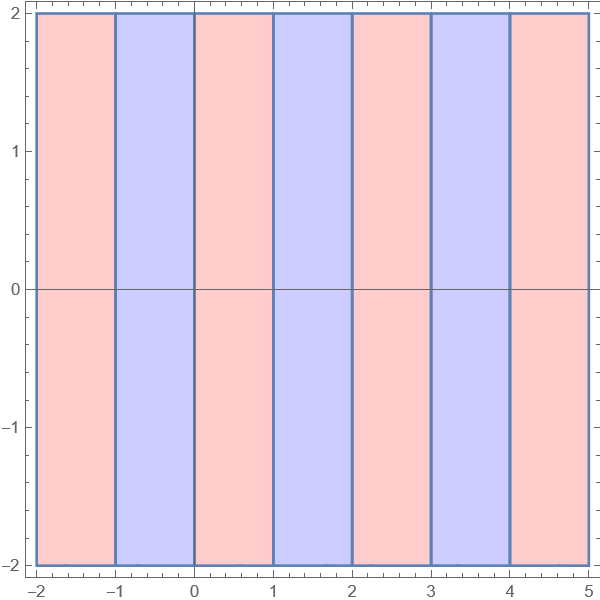
\includegraphics[scale=0.4]{no_square.png}
\end{center}
We claim there is no monochromatic copy of the four vertices of a unit square. If there were, then after a translation along $x$-direction, we can assume the unit square lie in $[0,3)\times \RR$ since the diagonal is $\sqrt{2}<2$. Let $(x_0,y_0)$ be the one with the smallest $x$-coordinate and $(x_2,y_2)$ with the largest, where the vertices are labeled counter-clockwise by $(x_0,y_0),(x_1,y_1),(x_2,y_2),(x_3,y_3)$. Say the angle between the $x$-axis and the  line joining $(x_0,y_0)$ and $(x_1,y_1)$ is $\alpha$. Then $0\leq \alpha \leq \pi/2$. In particular, we have \begin{align*}
  x_0 & = x_0                             \\
  x_1 & = x_0 + \cos{\alpha}              \\
  x_2 & = x_0 + \cos{\alpha}+\sin{\alpha} \\
  x_3 & = x_0 + \sin{\alpha}
\end{align*}
Note the distance between $(x_0,y_0)$ and $(x_2,y_2)$ is $\sqrt{2}$ and the labeling is so chosen that $x_2-x_0 \geq 1$. We mush have $x_0$ and $x_2$ lie in different strips. But note $|x_0-x_1|\leq 1$ and $|x_0-x_3|\leq 1$, so $x_0,x_1,x_3$ lie in the same strip. It is also true that $|x_2-x_1|\leq 1$ and $|x_2-x_3|\leq 1$, so $x_2,x_1,x_3$ lie in the same strip. We reach a contradiction.
\newpage

\noindent \textbf{Q6:}  Form lecture, we know that the volume of a ball in dimension $d$ is given by $$\vol{B^d(r)} =K_d r^d ,$$ where $K_d$ is some constant depending on $d$ only.

Say $\vol{C}=v$. We assume $C$ contains a small ball $B^d(x,\epsilon)\subset C\subset \RR^d$. We claim that $$C\subset B^d(x,  \frac{d! v}{K_{d-1}  \epsilon^{d-1}}).$$ And hence, $C$ is bounded. If the claim does not hold, we can find a point $y\in C$ such that $||x-y|| = h >  \frac{d! v}{K_{d-1}  \epsilon^{d-1}}$. Since $C$ is convex, $C$ contains $\conv{ B(x,\epsilon) \cup \{y\}}$. The hyperplane passing through $x$ perpendicular to $\overrightarrow{xy}$ intersects with $B^d(x,\epsilon)$ at a high dimensional disk $D^{d-1}(x,\epsilon)$ whose boundary is an equator of the ball. Then $C$ also contains $\conv{ D^{d-1}(x,\epsilon) \cup \{y\}}$, which is a high dimensional cone with base disk $D^{d-1}(x,\epsilon)$ and height $h$. The volume of the cone is given by integration $$\vol{  \conv{ D^{d-1}(x,\epsilon) \cup \{y\}}} = \int_{0}^h   K_{d-1} (\frac{t}{h} \epsilon)^{d-1} dt   = \frac{K_{d-1} \epsilon^{d-1}
  }{d!} h < \vol{C}=v.$$
But then $h < \frac{d! v}{K_{d-1}  \epsilon^{d-1}}$. Contradiction.

\newpage

\noindent \textbf{Q7:}
I notice this is Exercise 2.1.1 in Matou\v{s}ek's book and find that it quickly follows from Exercise 2.1.2, which is credited to Blichtfeld and van der Corput in the book:

\begin{theorem}[Blichtfeld's theorem]
  If $S$ is a bounded measurable set of $\RR^d$ and $\vol{S}>k$, then there are points $s_0,\dots,s_{k}\in S$ with all $s_0-s_i\in \ZZ^d$. In other words, there is a vector $v$ such that $v+S$ contains at least $k+1$ lattice points.
\end{theorem}
\noindent The proof will be given later. Note the case $k=1$ is actually called Blichtfeld's principle in the course notes. Let us use this theorem to prove our problem.\\



Back to this problem. Take any $x, y \in \frac{1}{2} C$, which means $x=\frac{x'}{2}, y=\frac{y'}{2}$ for some $x',y'\in C$. Then $x+y=\frac{x'}{2} +\frac{y'}{2}$ is a convex combination of $x',y'\in C$. Since $C$ is convex, we have $x+y\in C$ and so $\frac{1}{2}C+\frac{1}{2}C \subset C$. Now $\vol{\frac{1}{2} C} = \frac{1}{2^d} \vol{C} > k$. By Blichtfeld's theorem, there are distinct points $s_0,\dots,s_k \in \frac{1}{2}C$ such that each $s_0-s_i \in \ZZ^d$ for $i=0,\dots,k$. Note that $ s_0+\frac{1}{2} C \subset \frac{1}{2} C+\frac{1}{2} C\subset C$ and $\frac{1}{2} C$ is centrally symmetric. Therefore, for each $i=1,\dots,k$, we have the lattice point $$s_0-s_i = s_0+(-s_i)\in s_0+\frac{1}{2} C\subset C.$$ There are $k$ of them and so by symmetry, $C$ contains at least $2k$ lattice points (other than the origin).\\


\begin{proof}[Proof of Blichtfeld's theorem]

  I did not figure out how to prove this. Here is the proof from \cite{old}.


  Let $f(x)=\sum_{y\in \ZZ^d} 1_{S+x}(y)$, that is, $f(x)$ is the number of lattice points in the translation $S+x$. Since $S$ is bounded and measurable, $f(x)$ is also measurable. Because the Lebesgue measure is inner regular, we have
  \begin{align*}
    \int_{[0,1]^d} f(x) dx & =\sum_{y\in\ZZ^n} \int_{[0,1]^d} 1_{S+x}(y)dx  \\
                           & = \sum_{y\in\ZZ^d} \int_{[0,1]^d} 1_{S}(y-x)dx \\
                           & = \sum_{y\in\ZZ^d} \int_{y-[0,1]^d} 1_{S}(t)dt \\
                           & =\int_{\RR^d} 1_{S}(t)dt = \vol{S} >k.
  \end{align*}
  Thus, $\max_{x\in [0,1]^d} f(x) \geq k+1$. We are done.

  The proof above can be interpreted in a geometrical way. The lattice points $\ZZ^d$ divide $\RR^d$ into cubes and so divide $S$ into $S_1,\dots,S_n$, each lying in its corresponding cube $R_1,\dots,R_n$. Now by a translation by a vector $x_i \in \ZZ^d$, we can move each $R_i$ to $[0,1]^d$. And in the meantime, $S_1,\dots,S_n$ are also translated into their congruent $S_1',\dots,S_n'$ in $[0,1]^d$. We claim some point in $[0,1]^d$ is covered by $S_1',\dots,S_n'$ more than $k$ times. If not, then the combined areas of these parts could not exceed $k$. Consequently, the combined areas  of the parts $S_1,\dots,S_n$, when translated back to their original positions in $S$ would not exceed $k$. Call this point $v$. Then $|(v+\ZZ^d)\cap C| >k$. In particular, $s_i=v+x_{i_j}$ for $i=0,\dots,k$ and some $x_{i_0},\dots, x_{i_k}$.
\end{proof}


\begin{thebibliography}{9}
  \bibitem{old}
  C.D. Olds, A. Lax, and G. Davidoff, \emph{The Geometry of Numbers}, The Anneli Lax New Mathematical Library, vol. 41, The Mathematical Association of America, 2000.
\end{thebibliography}




\end{document}
